% Owners: Cosmin (laptop), Sergiu (Hábrók counters)
\section{Performance analysis}
\label{sec:analysis}

\paragraph{Baseline.} On \texttt{kron20}, the original \gapbs{} with the default number of
threads needs \SI{8.58}{ms} per search on the laptop (median, IQR \SI{4.77}{ms},
\SI{1.83}{GTEPS}) and \SI{2.85}{ms} on Hábrók (IQR \SI{1.43}{ms}, \SI{5.51}{GTEPS}). The Hábrók
node has 12.8 times more cores and 20 times more memory bandwidth, but it is only 3 times
faster. The main question of our analysis is why.

\paragraph{Hotspots.} Table~\ref{tab:hotspots} shows where the laptop spends its time,
measured with perf sampling (about \num{46000} samples, 64 searches, all threads).
\begin{table}[ht]
\centering\small
\caption{Laptop, perf sampling (task-clock, \SI{5}{kHz}), \texttt{kron20}, 64 searches including loading the graph.}
\label{tab:hotspots}
\begin{tabular}{@{}lrl@{}}
\toprule
Function & Samples & What it does \\
\midrule
OpenMP runtime (\texttt{libgomp}) & \SI{50.0}{\percent} & threads waiting at barriers \\
\texttt{BUStep} & \SI{35.8}{\percent} & bottom-up step \\
\texttt{InitParent} & \SI{5.7}{\percent} & initialisation of every search \\
\texttt{TDStep} & \SI{3.1}{\percent} & top-down step \\
\texttt{BitmapToQueue} + \texttt{QueueToBitmap} & \SI{2.4}{\percent} & frontier conversion \\
\texttt{DOBFS} (last loop) and rest & \SI{3.0}{\percent} & \\
\bottomrule
\end{tabular}
\end{table}
Half of all CPU time is spent by threads that wait in the OpenMP runtime. One search has
about ten short parallel regions (Section~\ref{sec:app}) and each of them ends with a barrier.
The work inside them is not balanced: Kronecker graphs have a few vertices with a very high
degree, and in bottom-up the cost of a vertex depends on how fast it finds a neighbour in
the frontier. Of the useful work, \texttt{BUStep} is by far the biggest part. With
\texttt{perf annotate} (\texttt{pe/results/wsl/perf\_annotate\_all.txt}) we looked at the
instructions of \texttt{BUStep}. \SI{39}{\percent} of its samples are on the instruction just
after the load of the first neighbour ID. With timer sampling, the sample usually lands on
the instruction that uses the result of a slow load, so this is the cache miss at the start
of every neighbour list. Another \SI{11}{\percent} are on the bit test of the bitmap and about
\SI{13}{\percent} on loads of the CSR index. So the time is spent on memory accesses, not on
computation.

\paragraph{Hardware counters per function (Hábrók).} With PAPI regions we can measure every
function separately, which sampling on the laptop cannot do (Table~\ref{tab:papi}). We used one
thread, so that every region is fully counted.
\begin{table}[ht]
\centering\small
\caption{PAPI per function, Hábrók, 1 thread, \texttt{kron20}, per search (64 searches).
Misses are the generic event \texttt{PERF\_COUNT\_HW\_CACHE\_MISSES}.}
\label{tab:papi}
\begin{tabular}{@{}lrrrrr@{}}
\toprule
Function & Cycles [M] & Share & IPC & Cache misses [k] & Misses per unit of work \\
\midrule
\texttt{BUStep} & 64.0 & \SI{77.7}{\percent} & 0.77 & 532 & 0.32 per checked vertex \\
\texttt{InitParent} & 11.6 & \SI{14.0}{\percent} & 0.89 & 3.7 & - \\
\texttt{TDStep} & 3.6 & \SI{4.4}{\percent} & 1.01 & 216 & 0.75 per examined edge \\
\texttt{BitmapToQueue} & 2.4 & \SI{2.9}{\percent} & 4.80 & 0.2 & - \\
\texttt{QueueToBitmap} & 0.8 & \SI{0.9}{\percent} & 1.59 & 2.5 & - \\
\bottomrule
\end{tabular}
\end{table}
Even without any synchronisation, \texttt{BUStep} takes \SI{78}{\percent} of the cycles. Both
steps run at an IPC of about 1, while the core could do several instructions per cycle. In
\texttt{TDStep}, \SI{75}{\percent} of the examined edges give a cache miss, which is what we
expect for the random accesses to \texttt{parent[v]}. In \texttt{BUStep} only a third of the
checked vertices give a miss. The neighbour lists of vertices that follow each other are next
to each other in the CSR array, so the hardware prefetcher can load many of them in time. The
two conversion functions are simple bit operations with a high IPC, and they cost very little.

Branches also cost time. With one thread a search has 17.8 million branches, and 2.3 million
of them are mispredicted (\SI{12.9}{\percent}, measured with pecount). Most of them come from
the bit test and the early exit in \texttt{BUStep}, which depend on the data. A misprediction
typically costs 10 to 20 cycles, so this can be a large part of the 87 million cycles of a
search, although part of it overlaps with the waiting for memory.

The data TLB is not a problem on Hábrók: transparent huge pages are always on there, and one
search only has about \num{4200} dTLB misses, compared to about 2 million random accesses. We
also measured the counters with 128 threads, but these runs include the five slow first
searches, which take most of the run time, so we do not use these numbers.

\paragraph{Scaling with the number of threads.} Figure~\ref{fig:scaling} shows the time per
search for different numbers of threads. On the laptop the best time is with 8 threads
(\SI{8.39}{ms}). With 10 threads it is not faster, and the IQR becomes much larger
(\SI{12.3}{ms}). On Hábrók the time goes down until 48 to 64 threads that are bound to
neighbouring cores (\SI{1.38}{ms}, \SI{11.4}{GTEPS}), and then it goes \emph{up} again, to
\SI{3.53}{ms} with 128 threads. With \texttt{OMP\_PROC\_BIND=close}, 64 threads fill exactly
one socket. When the second socket is used, \texttt{parent} and the bitmaps have to be kept
coherent between the two sockets, more threads have to meet at every barrier, and every
thread has less work. Without binding, the best time is \SI{2.45}{ms} with 48 threads.

\begin{figure}[ht]
\centering
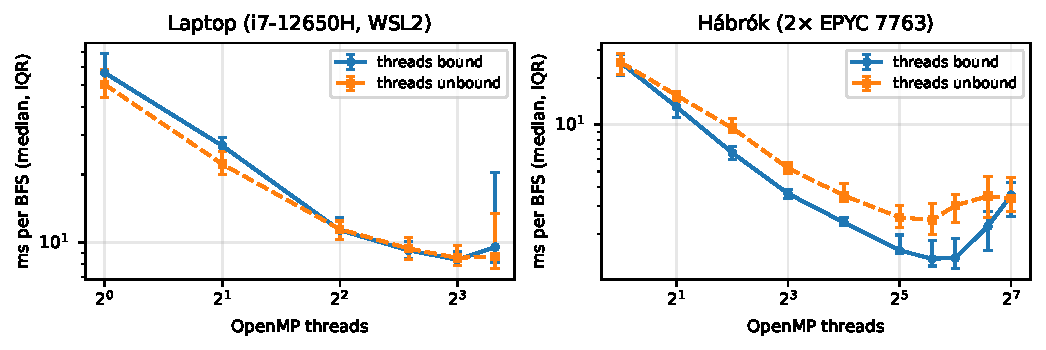
\includegraphics[width=\linewidth]{figures/scaling.pdf}
\caption{Time per search on \texttt{kron20} against the number of OpenMP threads, with the
threads bound to neighbouring cores (\texttt{OMP\_PROC\_BIND=close},
\texttt{OMP\_PLACES=cores}) and not bound (median, error bars: IQR).}
\label{fig:scaling}
\end{figure}

\paragraph{Memory hierarchy.} Figure~\ref{fig:latency} shows the latency of dependent loads on
both machines, measured with a pointer chase over a random cycle. The steps show the cache
sizes. On Hábrók the latency stays at 13 to \SI{15}{ns} up to \SI{32}{MiB} (the L3 of one
CCD) and is about \SI{99}{ns} in main memory. On the laptop it goes up to \SI{376}{ns} at
\SI{1}{GB}, probably because of TLB misses with nested paging. The working set of one
\texttt{kron20} search is about \SI{180}{MB} (Section~\ref{sec:model}). This is bigger than
all caches of the laptop. On Hábrók it is bigger than the L3 of one CCD, but would fit in all
16 L3 slices together. A core can only use the L3 of its own CCD, so data cached by another
CCD probably has to come over the interconnect, with a latency close to main memory.

\begin{figure}[ht]
\centering
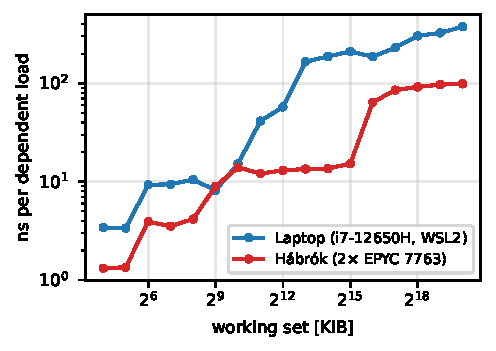
\includegraphics[width=0.55\linewidth]{figures/latency.pdf}
\caption{Latency of dependent loads against the size of the working set (one core).}
\label{fig:latency}
\end{figure}
